\section{Часть 1. Эксперимент}
\captionsetup{
	font=small,          % Уменьшает шрифт самой подписи
	labelfont={small}    % Уменьшает шрифт метки "Рисунок"
}

\subsection{Исспледование ВАХ полупроводниковых диодов на модели лабораторного стенда в программе microcap}

	\noindent Для заданного Мне диода \texttt{D2d2998d} провел моделирование лабораторного стенда и получил ВАХ диода в программе Microcap как на прямой ветви, так и на
	обратной ветви по указанным ниже схемам рис.1.
	\begin{figure}[ht]
		\centering
		\begin{subfigure}{0.45\textwidth}
			\centering
			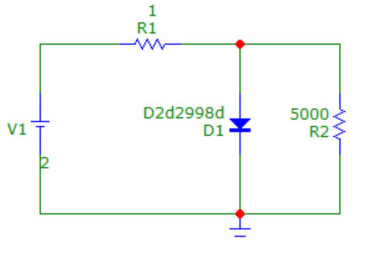
\includegraphics[width=\textwidth]{img/01_main_mcp.jpg}
			\caption{Прямая цепь}
			\label{fig:subfig_a}
		\end{subfigure}
		\hfill
		\begin{subfigure}{0.45\textwidth}
			\centering
			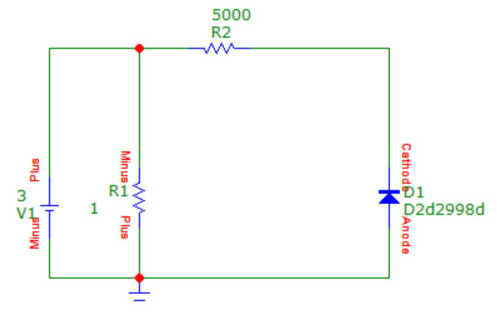
\includegraphics[width=\textwidth]{img/01_back_mcp.jpg}
			\caption{Обратная цепь}
			\label{fig:subfig_b}
		\end{subfigure}
		\captionsetup{font=footnotesize}
		\caption{Лабораторный стенд}
	\end{figure}
	
	\noindent Характеристики диода представлены на рис. \ref{fig:02_main_mcp}
	
	\begin{figure}[ht]
		\centering
		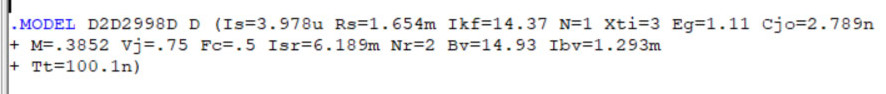
\includegraphics[width=0.9\textwidth]{img/02_main_mcp.jpg}
		\captionsetup{font=footnotesize}
		\caption{Характеристики диода}
		\label{fig:02_main_mcp}
	\end{figure}
	
	
	\noindent Затем я построил графики в microcap для схем прямого и обратного тока. В формуле на рис.3. I(RMA) домножил на 1 для получения напряжения по закону Ома. Затем нажал на кнопку \texttt{Run} для того, чтобы получить графики зависимости силы тока от напряжения
	\begin{figure}[ht]
		\centering
		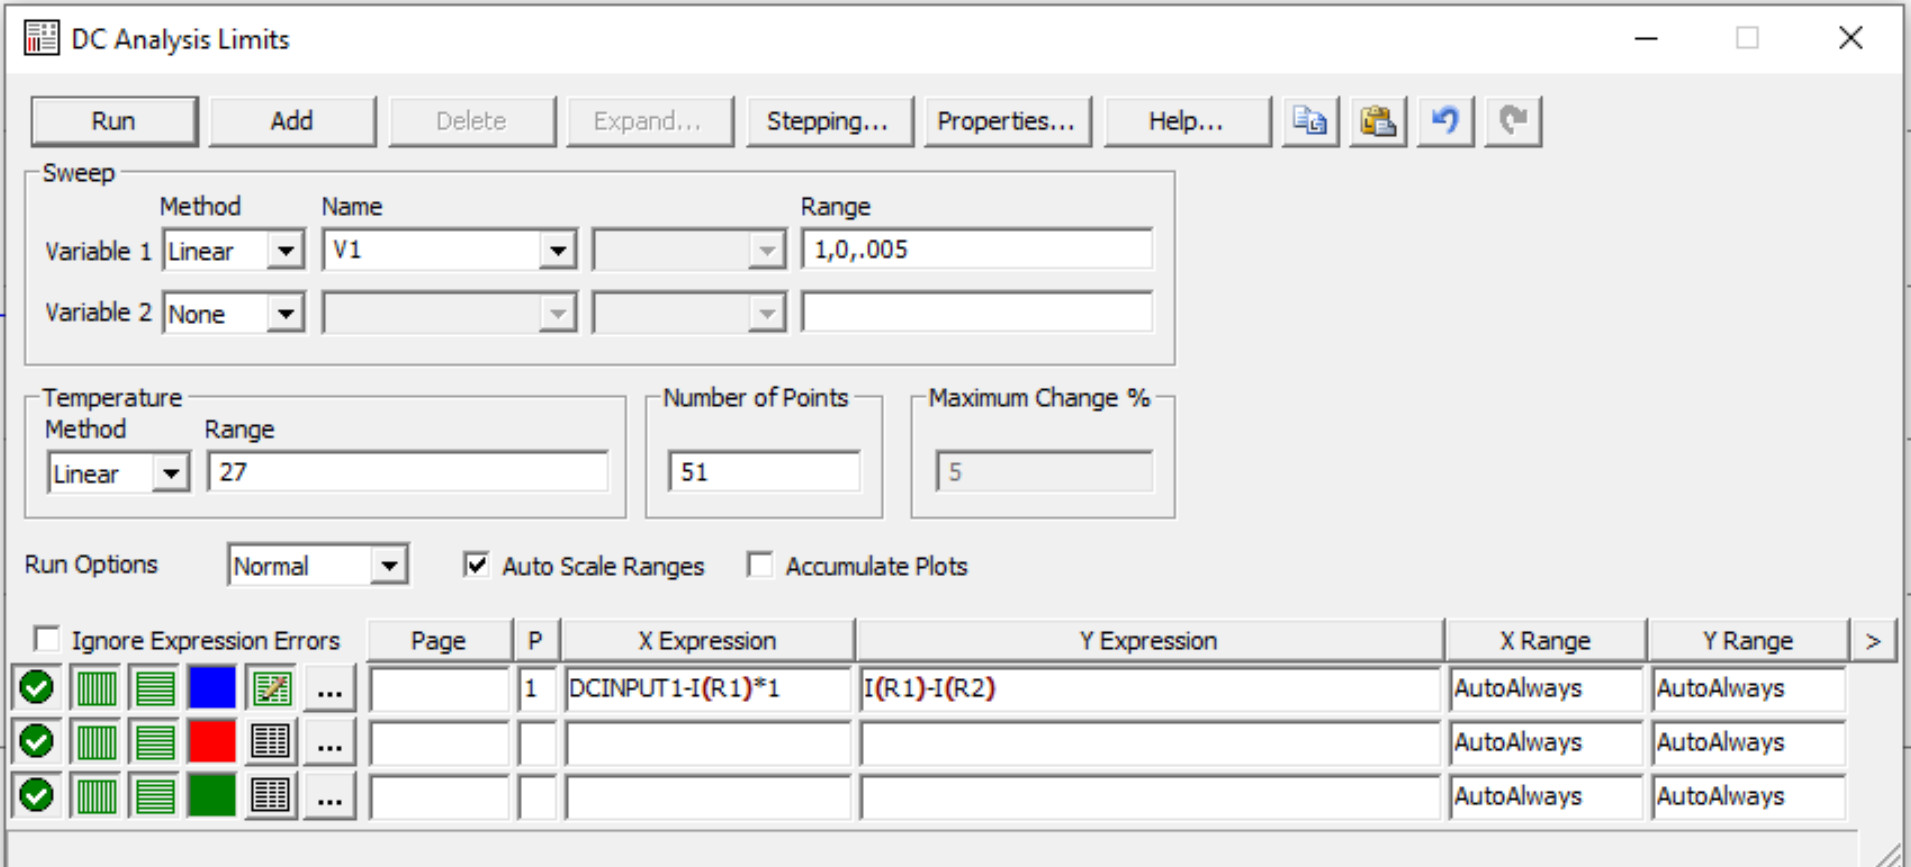
\includegraphics[width=0.9\textwidth]{img/05_main_mcp.jpg}
		\captionsetup{font=footnotesize}
		\caption{Аналитические данные прямой цепи}
		\label{fig:05_main_mcp}
	\end{figure}
	\begin{figure}[ht]
		\centering
		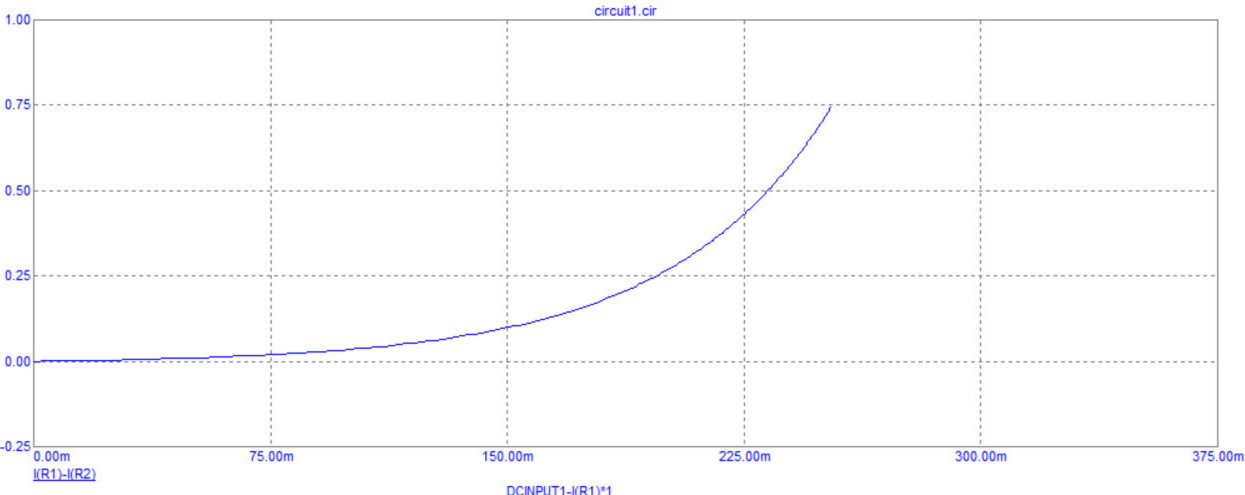
\includegraphics[width=0.9\textwidth]{img/03_main_mcp.jpg}
		\captionsetup{font=footnotesize}
		\caption{Зависимость прямого тока от напряжения}
		\label{fig:03_main_mcp}
	\end{figure}
	\begin{figure}[ht]
		\centering
		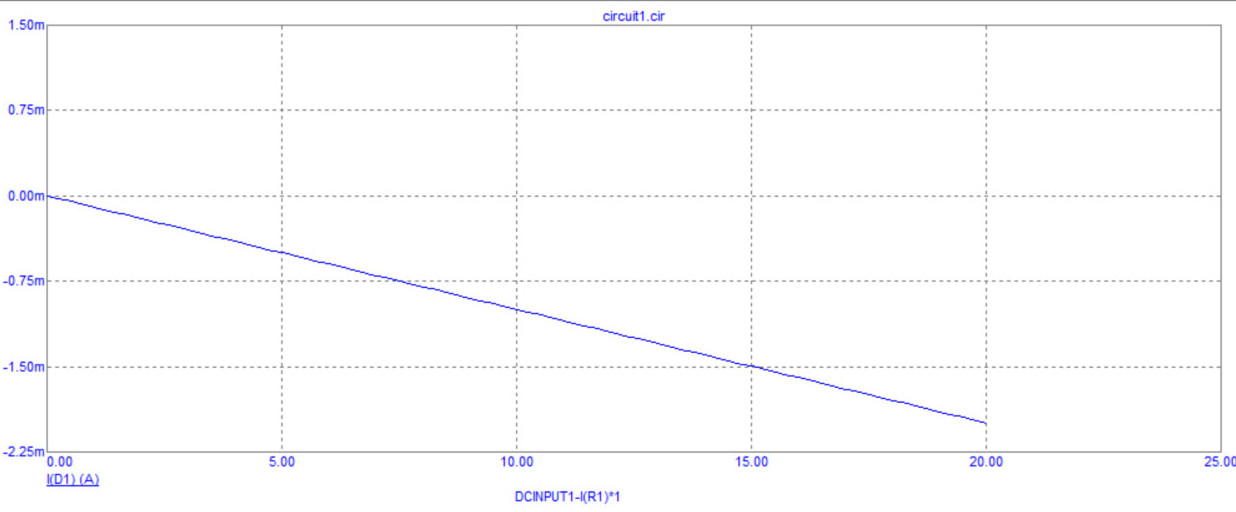
\includegraphics[width=0.9\textwidth]{img/02_back_mcp.jpg}
		\captionsetup{font=footnotesize}
		\caption{Зависимость обратного тока от напряжения}
		\label{fig:02_back_mcp}
	\end{figure}
	\clearpage
	\noindent Для прямого тока сделал вывод данных в текстовый файл, но перед этим убрал любую дополнительную информацию рис\ref{fig:06_main_mcp}: 
	\begin{figure}[H]
		\centering
		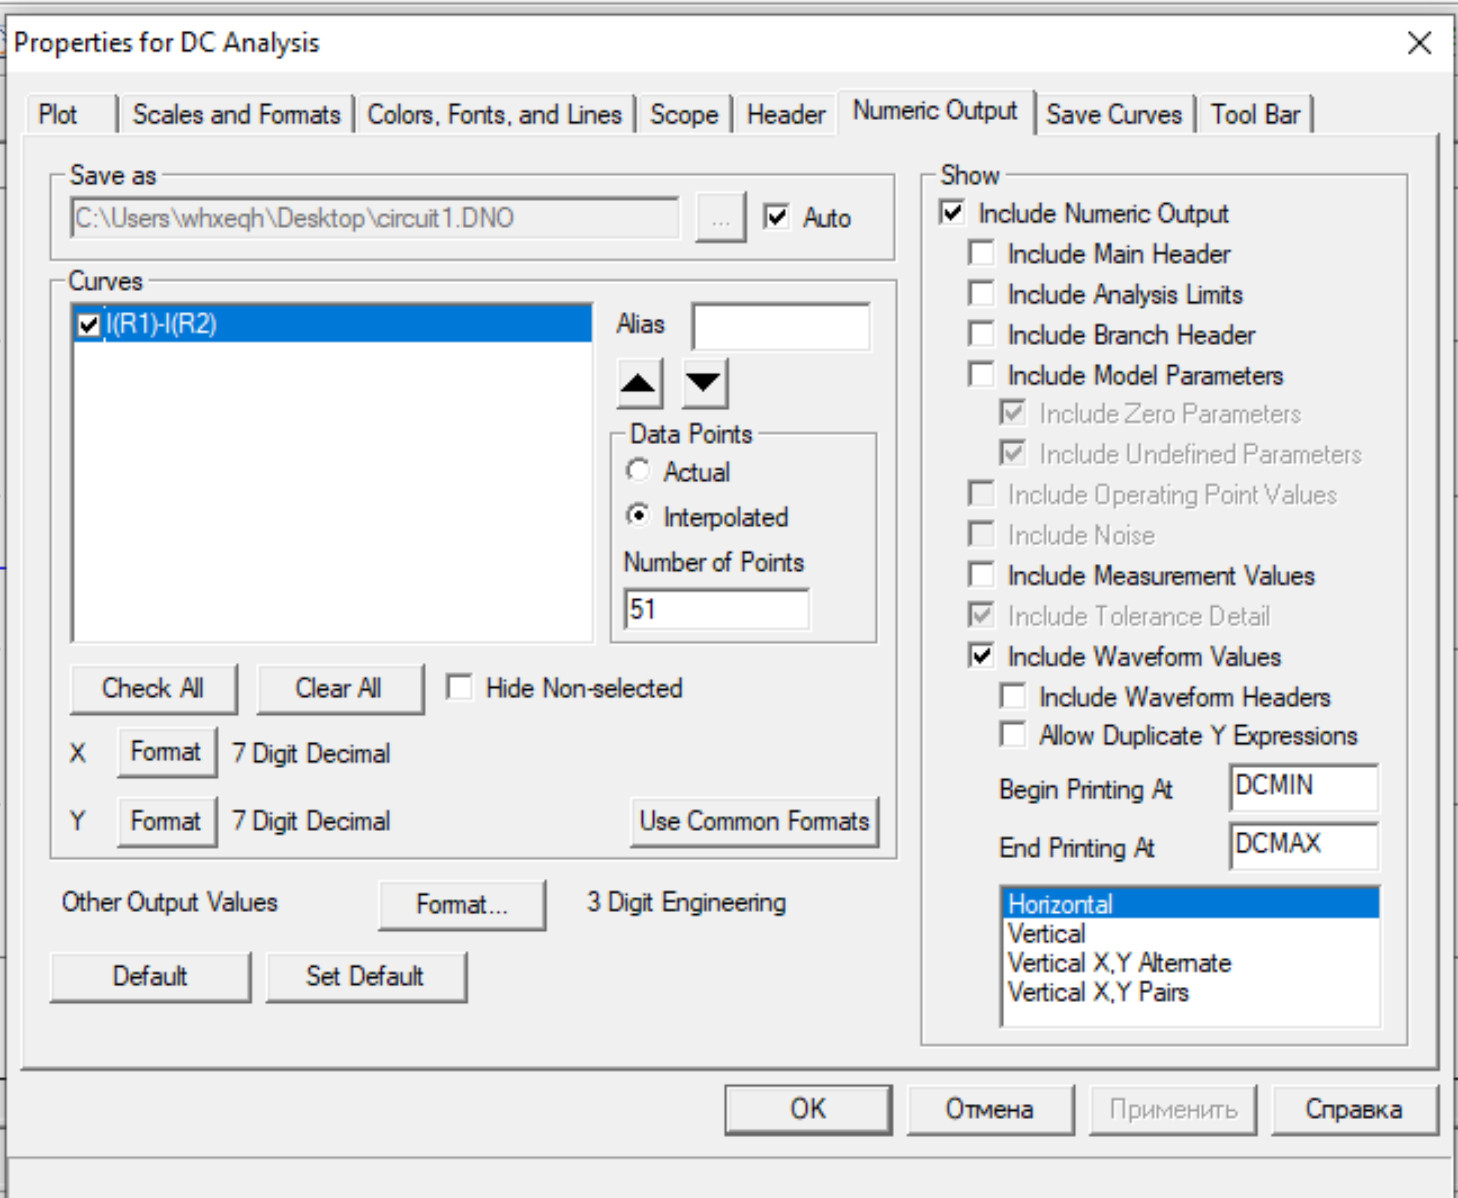
\includegraphics[width=0.5\textwidth]{img/06_main_mcp.jpg}
		\captionsetup{font=footnotesize}
		\caption{Окно Analysis/DC/limits}
		\label{fig:06_main_mcp}
	\end{figure}
	\noindent Итоговый текстовый файл с данными ВАХ:
	\begin{figure}[H]
		\centering
		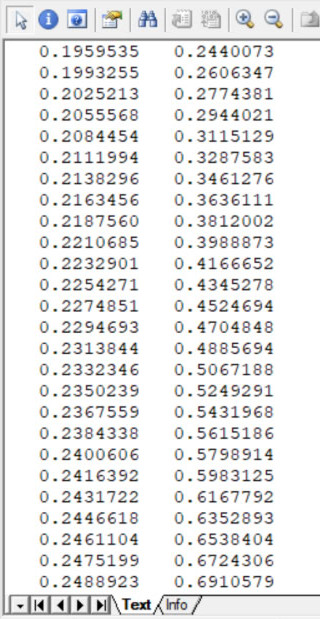
\includegraphics[width=0.3\textwidth]{img/04_main_mcp.jpg}
		\captionsetup{font=footnotesize}
		\caption{Сила тока и напряжение}
		\label{fig:04_main_mcp}
	\end{figure}
\newpage
\subsection{Обработка данных в mathcad}
\noindent Сначала я считал данные из полученного в \texttt{microcap} файла с помощью \texttt{READPRN}, разбил их на два отдельных столбца и построил график 

\begin{figure}[H]
	\centering
	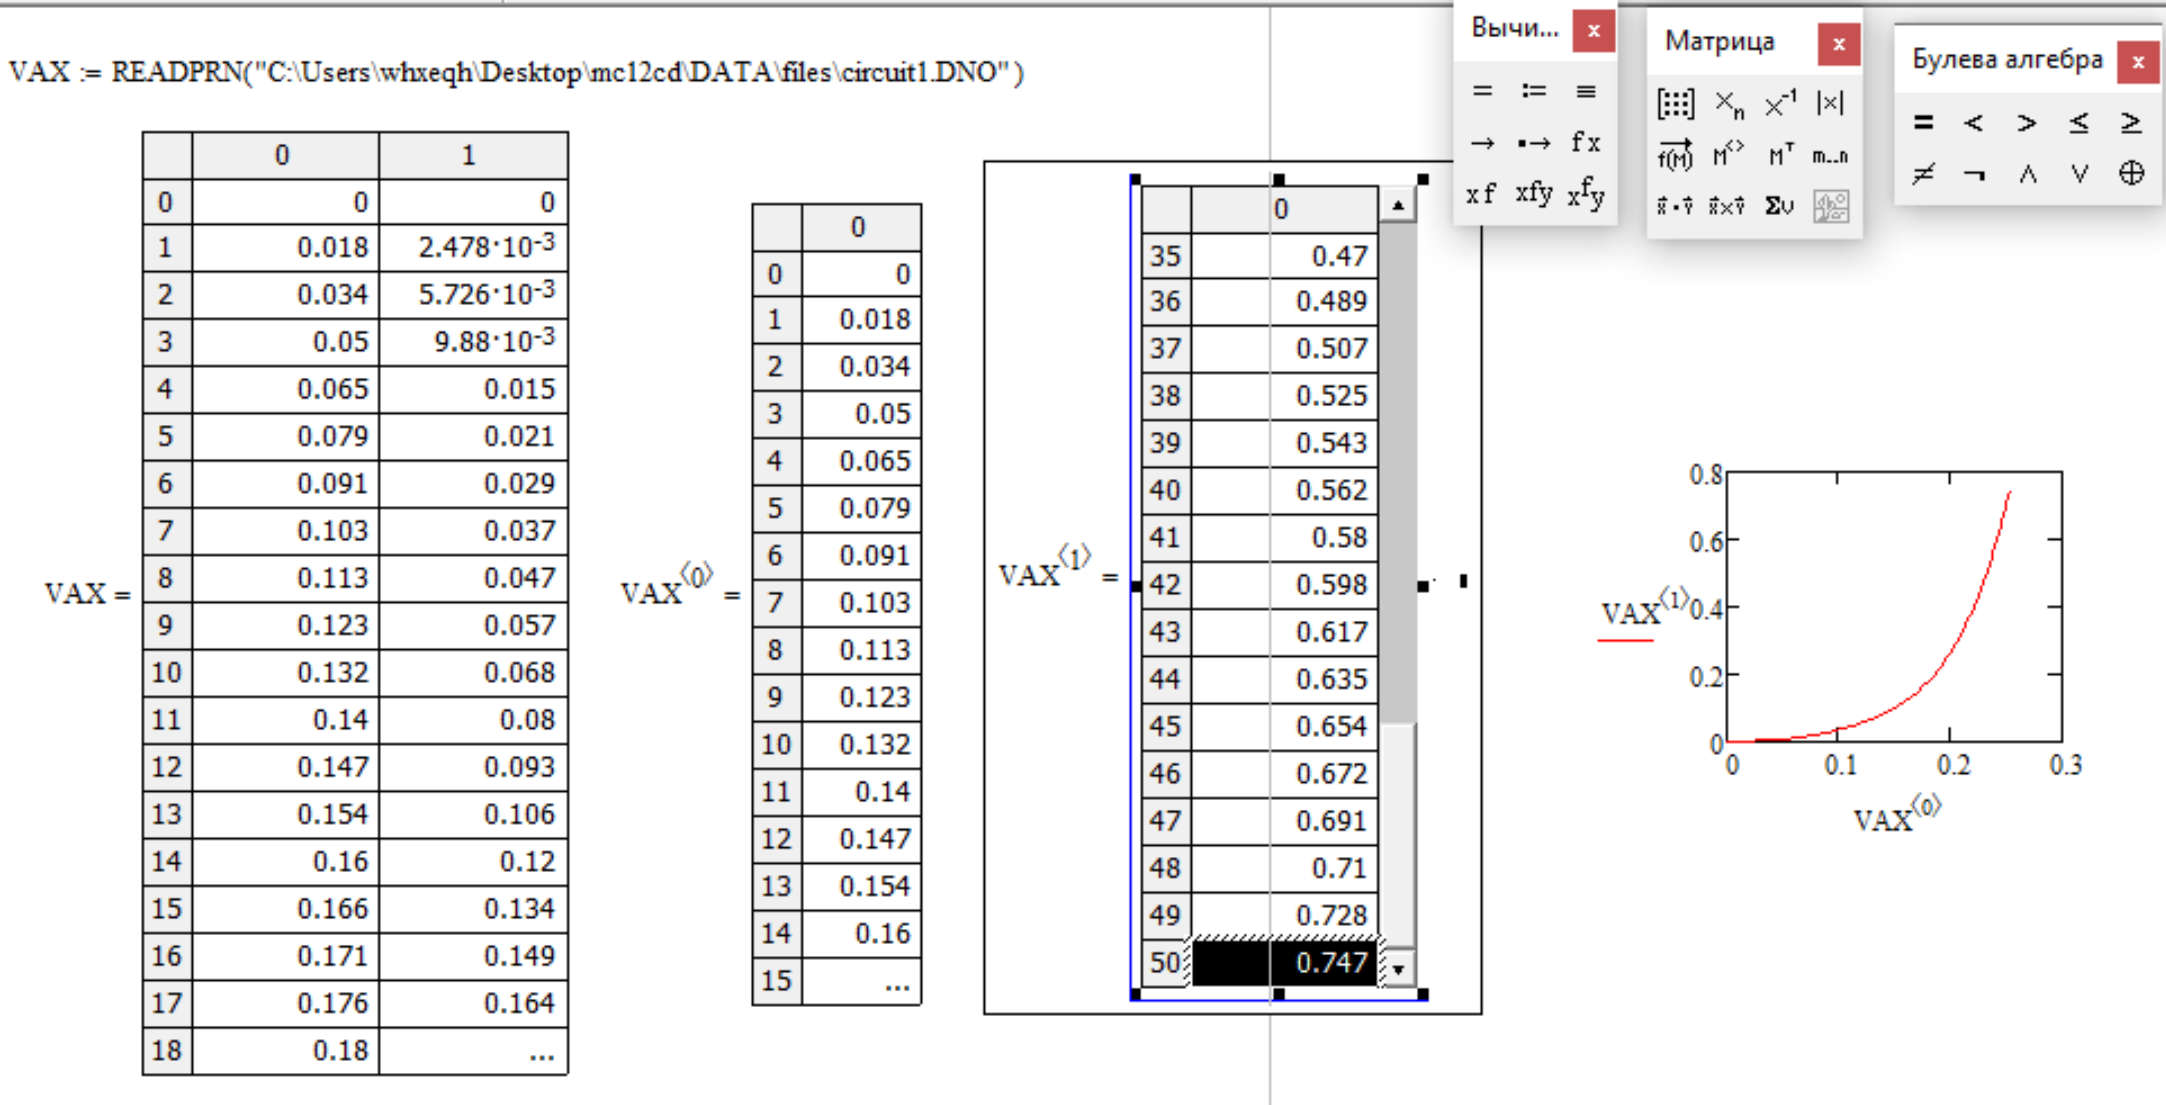
\includegraphics[width=0.98\textwidth]{img/01_mathcad.jgp}
	\captionsetup{font=footnotesize}
	\caption{Парсинг данных из microcap и построение графика}
	\label{fig:01_mathcad}
\end{figure}

\noindent Нашел параметры диода благодаря формулам из методички. 4 точки на графике искал методом трассировки 
\begin{figure}[H]
	\centering
	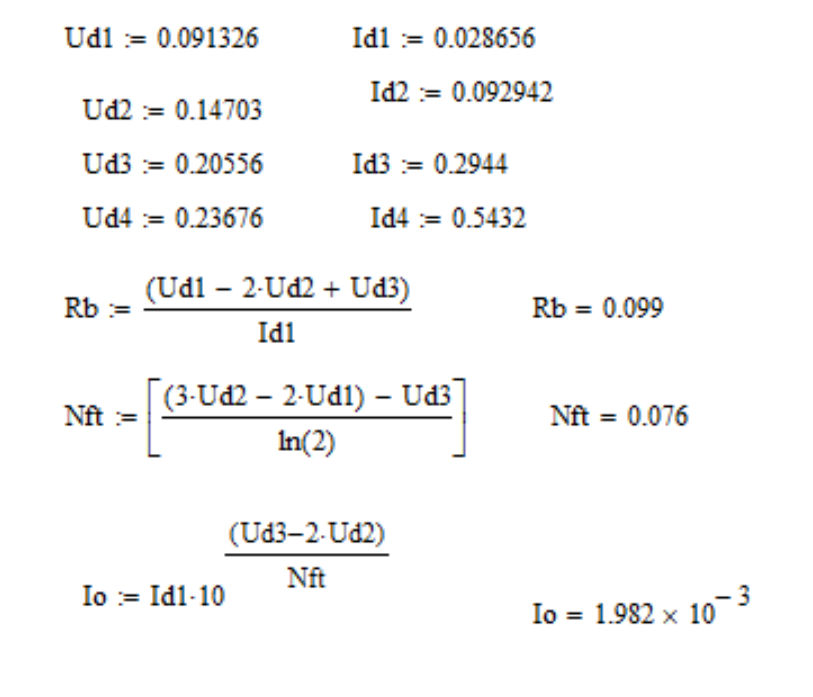
\includegraphics[width=0.63\textwidth]{img/02_mathcad.jgp}
	\captionsetup{font=footnotesize}
	\caption{Нахождение параметров диода}
	\label{fig:02_mathcad}
\end{figure}

\newpage
\noindent Затем нашел параметры модели полупроводникового диода методом \textbf{GIVEN MINERR}
\begin{figure}[H]
	\centering
	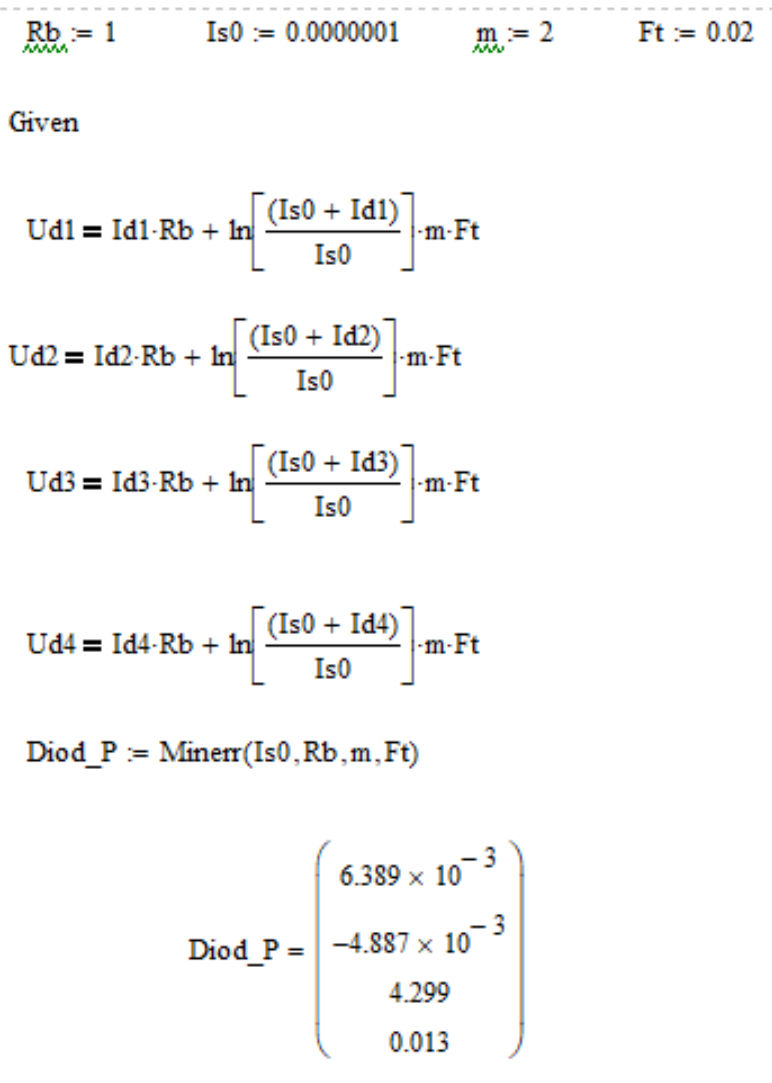
\includegraphics[width=0.4\textwidth]{img/03_mathcad.jgp}
	\captionsetup{font=footnotesize}
	\caption{Метод Given Minerr}
	\label{fig:03_mathcad}
\end{figure}
\noindent В итоге построил график ВАХ диода по формуле. Как видно из рис.\ref{fig:01_mathcad} мое максимальное значение силы тока \texttt{Idiod=0.747 А}
\begin{figure}[H]
	\centering
	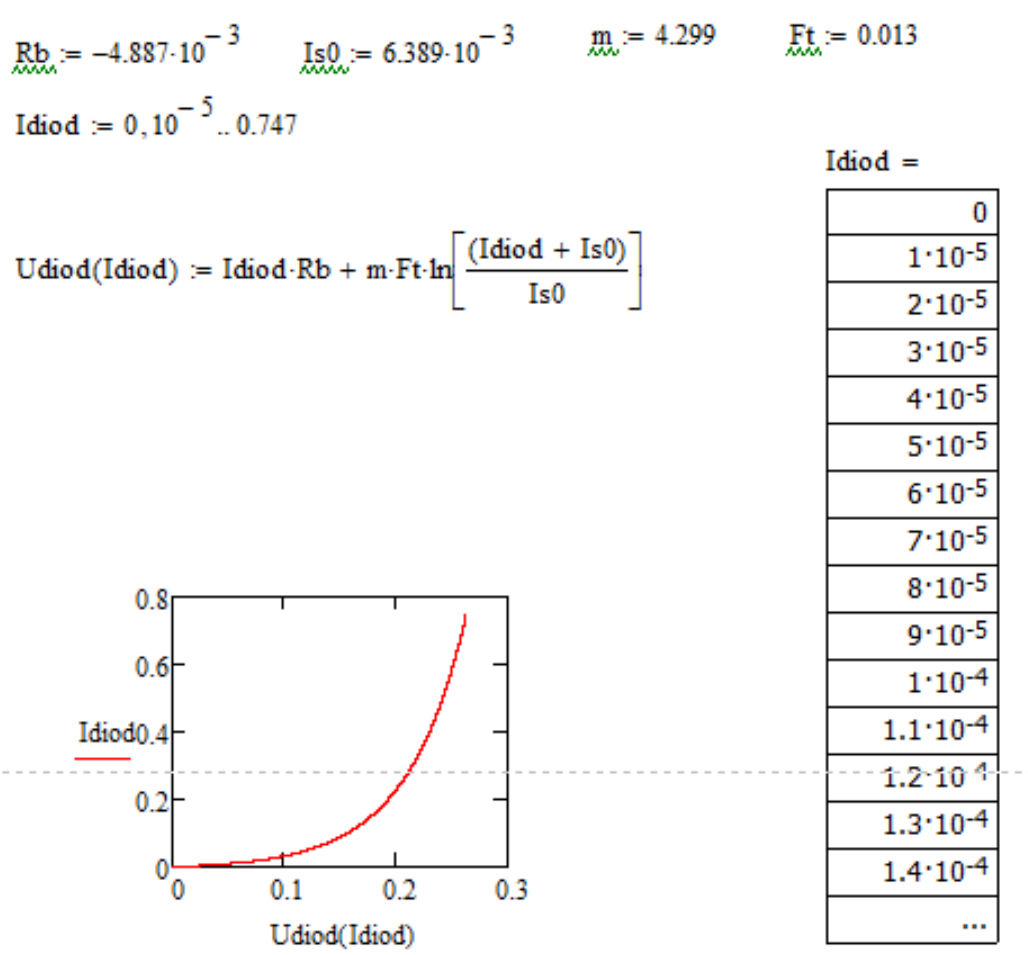
\includegraphics[width=0.6\textwidth]{img/04_mathcad.jpg}
	\captionsetup{font=footnotesize}
	\caption{График ВАХ диода}
	\label{fig:04_mathcad}
\end{figure}

\noindent Взяв одну из точек на графике, проверил работу формулы 
\begin{figure}[H]
	\centering
	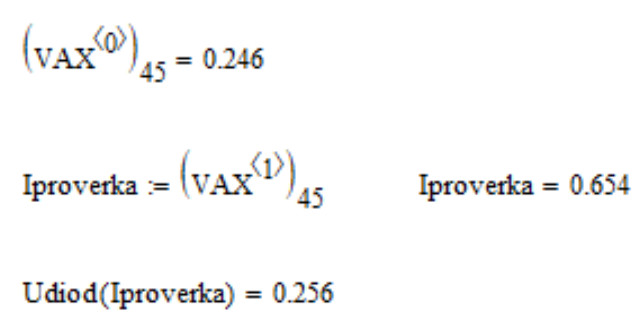
\includegraphics[width=0.45\textwidth]{img/05_mathcad.jgp}
	\captionsetup{font=footnotesize}
	\caption{Проверка формулы}
	\label{fig:05mathcad}
\end{figure}

\noindent Совместил ВАХ экспериментальную и ВАХ теоретическую на один график
\begin{figure}[H]
	\centering
	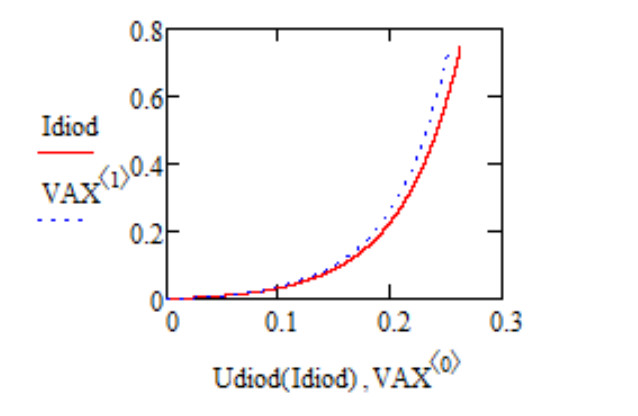
\includegraphics[width=0.45\textwidth]{img/06_mathcad.jgp}
	\captionsetup{font=footnotesize}
	\caption{Исходный и теоретический график}
	\label{fig:06mathcad}
\end{figure}
